\chapter{Requirements}
\label{ch:requirements}
\section{Requirements Elicitation}

To ensure that our system reflects real user needs, we have created several typical user roles and user stories. They cover different types of users, such as those who care about fashion trends, those who want to make quick decisions, system administrators, and those who focus on making better use of their wardrobe.

Due to limited space, detailed character roles and user stories are included in the Appendix~\ref{appendix:elicitation}. They helped us determine the main functions of the system, such as clothing recommendation, virtual try-on, wardrobe management, and analysis.

\section{Requirement Specification}
This section defines the functional and non-functional requirements for our system. Requirements are organized by module and assigned unique identifiers (FR-XX for functional, NF-XX for non-functional) to enable traceability across design, implementation, and testing phases.

\subsection{Functional Requirements}
Table \ref{tab:functional_requirements} below summarizes the functional requirements of the system. Each requirement is assigned a priority according to the MoSCoW method.

\begin{table}[h]
\centering
\caption{MoSCoW Priority Levels}
\label{tab:moscow}
\renewcommand{\arraystretch}{1.3} 
\begin{tabular}{lp{10cm}}
\toprule
\textbf{Priority} & \textbf{Definition} \\
\midrule
Must   & Core functionality essential for delivery \\
Should & Important functionality with acceptable alternatives \\
Could  & Optional features implemented if time permits \\
\bottomrule
\end{tabular}
\end{table}


\newpage
\begin{table*}[ht]
\centering
\small
\caption{Functional Requirements (FR)}
\label{tab:functional_requirements}
\renewcommand{\arraystretch}{1.2}
\begin{tabular}{p{2.8cm}p{1.6cm}p{9cm}p{1.4cm}}
    \toprule
    \textbf{Module} & \textbf{FR ID} & \textbf{Description} & \textbf{Priority} \\
    \midrule
    User Account Management & 
    FR-01 &
    The system must support user registration, login, logout, and initialize wardrobe setup after first login.  & 
    Must \\

          &
    FR-04 &
    The system must maintain a user preference profile and allow users to edit personal preferences.  &
    Should \\

    Wardrobe Management &
    FR-02 &
    The system must allow users to add clothing items via structured forms (basic attributes, metadata, photos). & 
    Must \\

          &
    FR-03 &
    The system must support batch image uploads and automatically generate candidate tags based on visual attributes.  &
    Should \\

          &
    FR-13 &
    The system must support wardrobe maintenance, including search, filtering, batch editing and deletion. &
    Must \\

    Recommendation System &
    FR-05 &
    The system must allow users to input outfit constraints, including occasion, etiquette, comfort level and color choices. &
    Must \\
    
          &
    FR-06 &
    The system must automatically retrieve weather conditions based on user location and date, with an option for manual override. & 
    Should \\
    
          &
    FR-07 &
    The system must generate no fewer than three outfit recommendations that satisfy occasion, weather and preference constraints. &
    Could \\
    
          &
    FR-08 &
    The system must provide explanation for each recommendation and offer alternative items or outfits for adjustment. &
    Should \\

          &
    FR-09 &
    The system must collect user feedback (like/dislike/avoid) and update preference learning for future recommendations. &
    Could \\
    
    Virtual Try-On &
    FR-10 &
    The system must allow users to upload full-body photos and preview outfit try-on results on their own images. &
    Must \\
    
          &
    FR-11 &
    The system must support try-on using clothing photos by segmenting and aligning garments for preview. & 
    Must \\
    
          &
    FR-12 &
    The system must support exporting or sharing try-on results in image format or via shareable links. &
    Could \\
    
    \bottomrule
\end{tabular}
\end{table*}

To improve testability and traceability, each functional requirement is associated with a planned validation method in Table~\ref{tab:FR_verification}. These methods indicate how each requirement can be checked during testing. The detailed testing process is presented in Chapter~\ref{ch:testing}, while Chapter~\ref{ch:evaluation} reports the final implementation status and verification results.

\newpage 
\begin{table*}[h]
\centering
\small
\caption{Verification Methods for Functional Requirements}
\label{tab:FR_verification}
\renewcommand{\arraystretch}{1.2}
\begin{tabular}{p{3.2cm}p{1.5cm}p{10cm}}
\toprule
\textbf{Module} & \textbf{FR ID} & \textbf{Verification Method} \\
\midrule

User Account Management 
& FR-01 
& Check that a user can create an account, log in successfully, log out, and that protected pages show an error or redirect when accessed without login. \\

& FR-04 
& Check that user preference data is displayed on the profile page and that changes remain after saving and refreshing the page. \\

Wardrobe Management 
& FR-02 
& Check that a new clothing item appears in the wardrobe list immediately after submission and remains after page reload. \\

& FR-03 
& Check that uploading multiple images shows all uploaded items and that generated tags are visible and selectable. \\

& FR-13 
& Check that search results change when keywords are entered, filters change the displayed items, and edited or deleted items are updated in the list. \\

Recommendation System 
& FR-05 
& Check that different input constraints (e.g., occasion or color) lead to different recommendation outputs. \\

& FR-06 
& Check that weather information changes when location changes and that manual override replaces the displayed weather. \\

& FR-07 
& Check that at least three recommendation items are displayed after submitting a valid request. \\

& FR-08 
& Check that explanation text appears under each recommendation and that selecting an alternative updates the displayed result. \\

& FR-09 
& Review system design to identify where user feedback (like/dislike) would be stored and how it could influence future recommendations. \\

Virtual Try-On 
& FR-10 
& Check that uploading a user image produces a new try-on image that is displayed on the page. \\

& FR-11 
& Check that the clothing region overlaps with the body region in the generated image and follows the body shape. \\

& FR-12 
& Review system design to identify how generated images could be downloaded or shared through links. \\

\bottomrule
\end{tabular}
\end{table*}


\subsection{Non-Functional Requirements}
Table \ref{tab:nfr} summarizes the non-functional requirements, covering performance, usability, security, reliability, and compatibility. Each requirement includes a quantifiable metric to enable objective validation.

\begin{table}[H]
\centering
\small
\caption{Performance requirements (NF)}
\label{tab:nfr}
\renewcommand{\arraystretch}{1.5}
\begin{tabular}{p{2.2cm}p{1.4cm}p{8.1cm}p{2.1cm}}
\toprule
\textbf{Category} & \textbf{NF ID} & \textbf{Brief Description} & \textbf{Quantifiable Metric}\\
\midrule
Performance & NF-01 & 95\% of requests complete within 3 seconds & $\leq$ 3 sec\\

 & NF-02 & System maintains stable response under load & $\geq$ 10 concurrent users \\

 & NF-03 & Single 720p image processed and displayed within 10 seconds & $\leq$ 10 sec\\

Usability & NF-04 & UI components follow defined design system (colors, fonts, spacing, component consistency) \\

 &NF-05 & Core functions (upload, recommendation, sharing) can be completed within 3 clicks/step & $\leq$ 3 steps\\

 & NF-06 & New users complete registration and wardrobe setup within 120 seconds & $\leq$ 2 minutes\\

 & NF-07 & All interface text switches correctly between Chinese and English & CN/EN switching\\

Security and Privacy & NF-08 & User-uploaded photos are not used for model training or shared with third parties &  Try-on only\\

 & NF-09 & Users can delete account; all associated data (photos, preferences, wardrobe) are permanently removed & Full data removal\\

Reliability & NF-10 & System operational for $\geq$ 99\% of time ($\leq$ 3.65 days downtime per year). & $\geq$ 99\% \\

 & NF-11 & Data saved prior to crash remains intact after system restart & No loss on crash\\

Compatibility & NF-12 & Core functions work correctly on all specified browsers & Chrome, Edge, Safari, Firefox\\

 & NF-13 & Core functions accessible on mobile devices & iOS / Android\\

\bottomrule
\end{tabular}
\end{table}

Table~\ref{tab:NFR_verification} explains how these requirements will be checked in practice. In this way, the non-functional requirements are not only defined by measurable targets, but are also linked to later testing and evaluation.

\newpage
\begin{table*}[h]
\centering
\small
\caption{Verification Methods for Non-Functional Requirements}
\label{tab:NFR_verification}
\renewcommand{\arraystretch}{1.2}
\begin{tabular}{p{1.8cm}p{11cm}}
\toprule
\textbf{NF ID} & \textbf{Verification Method} \\
\midrule

NF-01 & Measure response time over multiple requests and confirm that at least 95\% complete within 3 seconds. \\

NF-02 & Simulate multiple concurrent users and observe whether the system continues responding without failure. \\

NF-03 & Upload a 720p image and record the time from submission to result display. \\

NF-04 & Inspect different pages and confirm that colors, fonts, spacing, and layout are consistent. \\

NF-05 & Perform core tasks (upload, recommendation, sharing) and count the number of user interactions required. \\

NF-06 & Measure the time taken for a new user to complete registration and initial setup. \\

NF-07 & Switch language settings and verify that all interface text updates accordingly. \\

NF-08 & Review system design and data flow to confirm that uploaded images are not stored or used externally. \\

NF-09 & Delete a user account and verify that associated data is no longer accessible. \\

NF-10 & Monitor system uptime during operation and calculate availability percentage. \\

NF-11 & Simulate system restart and check that previously saved data remains available. \\

NF-12 & Run the system on different browsers and verify correct functionality. \\

NF-13 & Access the system on mobile devices and verify that core features are usable. \\

\bottomrule
\end{tabular}
\end{table*}

These methods show how each requirement will be checked in practice and will be used later in testing and evaluation.




\newpage
\subsection{Use Case Diagram and Descriptions}
\begin{figure}[H]
    \centering
    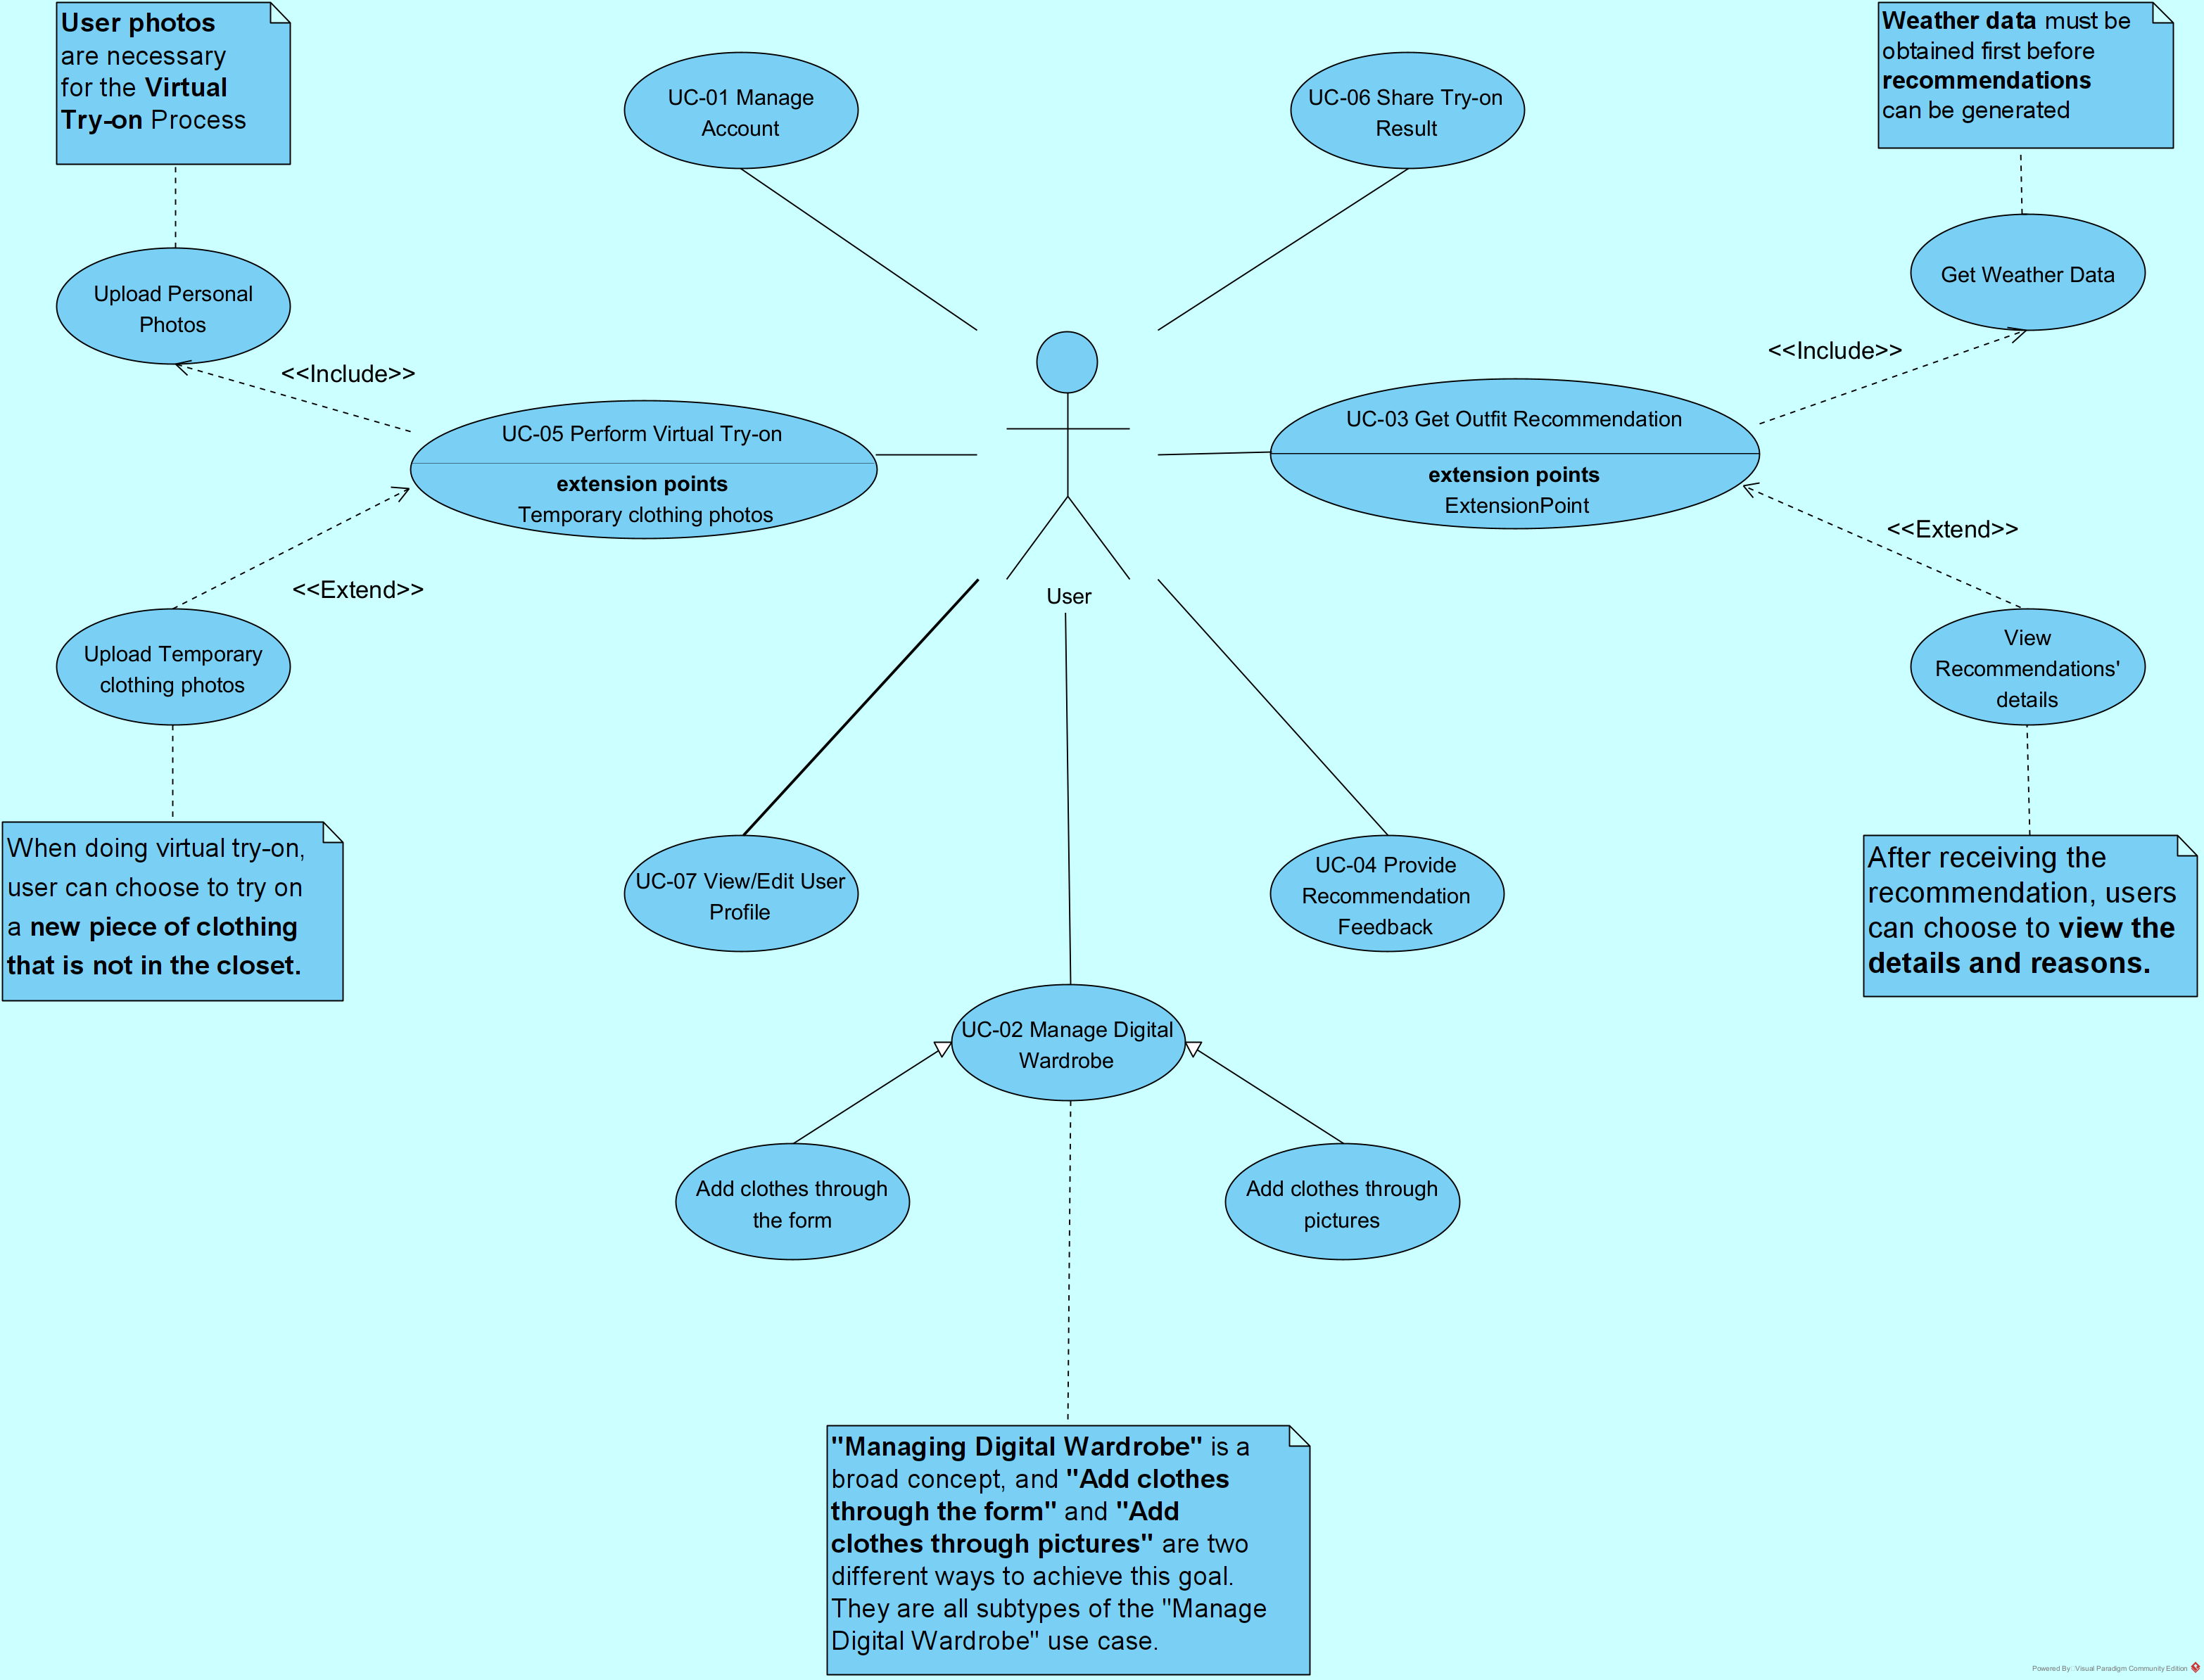
\includegraphics[width=1.0\textwidth]{images/Section_4_requirement/UCD.png}
    \caption{Use Case Diagram}
    \label{fig:UCD}
\end{figure}

Figure~\ref{fig:UCD} shows the overall functional structure of the system. The only actor is the "User." It presents the main use cases within the system boundary and the relationships between them.

The core use cases include: Manage Account, Manage Digital Wardrobe, Get Outfit Recommendation, Provide Recommendation Feedback, Perform Virtual Try-on, Share Try-on Result, and View/Edit User Profile.

Relationships between use cases are expressed through «include» and «extend». "Perform Virtual Try-on" includes "Upload Personal Photos." It also extends to "Upload Temporary Clothing Photos." This optional flow allows users to try on clothes not in their wardrobe.

"Get Outfit Recommendation" requires weather data before it can be executed. This shows a dependency on external information.

Under the goal of "Manage Digital Wardrobe," there are two ways to achieve it: add clothes through a form, and add clothes through pictures. The diagram presents them side by side. Both are specific ways to manage the digital wardrobe.

\newpage
Table~\ref{tab:uc_overview} below summarizes the seven core use cases of the system. They cover account management, wardrobe management, recommendation generation and feedback, virtual try-on, result sharing, and profile maintenance. They support the core business process of the virtual try-on system.
\begin{table}[H]
\centering
\caption{Use Case Overview}
\label{tab:uc_overview}
\renewcommand{\arraystretch}{1.5}
\begin{tabular}{p{4cm} p{12cm}}
\toprule
\textbf{Use Case ID} & \textbf{Brief Description} \\
\midrule
UC-01 Manage Account &
Users register, log in, or log out of the system. First-time users may complete initial wardrobe setup. \\
UC-02 Manage Digital Wardrobe &
Users add, edit, delete, and browse clothing items using forms or image uploads. The system processes and stores wardrobe entries. \\
UC-03 Get Outfit Recommendation &
The system generates personalized outfits based on preferences, weather, occasions, wardrobe items, and constraints, including explanations and alternatives. \\
UC-04 Provide Recommendation Feedback &
Users give feedback on recommendations (like/dislike/collect/not interested). The system updates preference models. \\
UC-05 Virtual Try-on &
Users upload photos or use wardrobe items to generate virtual try-on previews through body segmentation and overlay. \\
UC-06 Share Try-on Result &
Users export images or generate shareable links of their virtual try-on results. \\
UC-07 View/Edit User Profile &
Users view and edit preference profiles generated from wardrobe and interaction history. \\
\bottomrule
\end{tabular}
\end{table}


\newpage
To ensure that the requirements are not merely conceptual but operationalized in actual workflows, each use case is explicitly linked to one or more functional requirements.

The following traceability matrix serves as a validation mechanism. It provides bi-directional traceability, confirming that no requirement is left unsupported and no use case is functionally unjustified.

\begin{table}[H]
\centering
\caption{Functional Requirements -- Use Case Traceability Matrix}
\label{tab:fr_uc_matrix}
\small
\setlength{\tabcolsep}{3pt}
\renewcommand{\arraystretch}{1.5}
\begin{tabular}{p{4cm} | c c c c c c c}
\toprule
\textbf{Functional Requirement} &
\textbf{UC-01} &
\textbf{UC-02} &
\textbf{UC-03} &
\textbf{UC-04} &
\textbf{UC-05} &
\textbf{UC-06} &
\textbf{UC-07} \\
\midrule
FR-01 Account registration/login                 & X &   &   &   &   &   &   \\
FR-02 Wardrobe creation (Form)                   &   & X &   &   &   &   &   \\
FR-03 Wardrobe creation (Image)                  &   & X &   &   &   &   &   \\
FR-04 User preferences (profile)                 &   &   & X & X &   &   & X \\
FR-05 Occasion and constraint input              &   &   & X &   &   &   &   \\
FR-06 Weather data acquisition                   &   &   & X &   &   &   &   \\
FR-07 Outfit recommendation                      &   &   & X &   &   &   &   \\
FR-08 Explanation / alternatives                 &   &   & X &   &   &   &   \\
FR-09 Feedback loop \& learning                  &   &   &   & X &   &   &   \\
FR-10 Virtual try-on (user photo)                &   &   &   &   & X &   &   \\
FR-11 Virtual try-on (clothing image)            &   &   &   &   & X &   &   \\
FR-12 Share try-on results                       &   &   &   &   &   & X &   \\
FR-13 Wardrobe maintenance                       &   & X &   &   &   &   &   \\
\bottomrule
\end{tabular}
\end{table}


\section{Requirement Validation}
\textbf{\large a. Traceability Validation}

As shown in the Functional Requirements--Use Case Traceability Matrix
(Table~\ref{tab:fr_uc_matrix}), every functional requirement is linked to at least
one use case, and no use case exists without originating from a defined
requirement. This ensures bidirectional traceability: (i) each requirement is
implemented through at least one user workflow, and (ii) each workflow has a
clear requirement basis defined in the SRS. This validation step helps prevent
missing functionality and unjustified features.\\

\textbf{\large b. Supervisor Review and Confirmation}

The core modules of the system --- wardrobe management, wardrobe analysis, outfit recommendation, my calendar, and virtual try-on --- have been reviewed with the project supervisor and confirmed as the primary development priorities. During this review, the supervisor also verified that the main non-functional requirements are realistic and feasible under the current technical constraints.
    